In this section, we show the effectiveness of our approach on some examples,
and compare it to other existing approaches.
All computations except one ( \textsc{ASP-Thomas} ) were performed on a Pentium~V, 3.2~GHz with 4~GB RAM.

\subsection{Evaluation}
To assess the efficiency of our new approach,
we position ourselves with respect to existing methods dealing with different biological models.
We have chosen the following tools, that are detailed below: 
\textsc{GINsim}\footnote{\textsc{GINsim} \url{http://ginsim.org/}} (Gene Interaction Network Simulation)~\cite{gonzalez2006ginsim,naldi2009logical,naldi2007decision},
\textsc{LibDDD}\footnote{\textsc{LibDDD} \url{http://move.lip6.fr/software/DDD/}}
(Library of Data Decision Diagrams)~\cite{thierry2009hierarchical,colange2013towards},
\textsc{Pint}\footnote{\textsc{Pint} \url{http://loicpauleve.name/pint/}}~\cite{PMR12-MSCS}
and the method for CTL model-checking proposed by Rocca \textit{et al.} in~\cite{roccaasp},
which was developed also in ASP but for states transitions networks.
Each method uses a specific kind of representation\footnote{When available, we used the converters included into \textsc{Pint} for these translations.}:
Thomas models (a particular kind of logical regulatory networks) for \textsc{GINsim},
instantiable transition systems for \textsc{LibDDD},
state transition networks for the method of Rocca \textit{et al.}
and Process Hitting (PH) for \textsc{Pint} as well as for our method.

For this comparative study, we focus on biological network of different sizes:
a tadpole tail resorption (TTR) model with 12 biological components~\cite{khalis2009smbionet},
an ERBB receptor-regulated G1/S transition (ERBB) model with 20 components~\cite{Samaga2009}
and a T-cell receptor (TCR) signaling network of 40 components~\cite{Klamt06}.
These models were chosen to be of different sizes:
from small (12 components) to large (40 components).
We note however that the considered PH models may contain more sorts than
the original number of biological components, due to the use of
“cooperative sorts”, which allow to model Boolean gates but do not necessarily
have a biological meaning.
The different model representations that are required for performing these benchmarks have been obtained by translations
from the PH
ensuring the conservation of the dynamical properties.
All results alongside with more detailed specifications of the models
are given in table \ref{tab:reachability}.
The methods and the results provided by each of them are detailed in the following.
The overall results show that our method is efficient in computing reachability
from a given initial state;
furthermore, it sometimes provides more information than the other existing ones.

\begin{table}

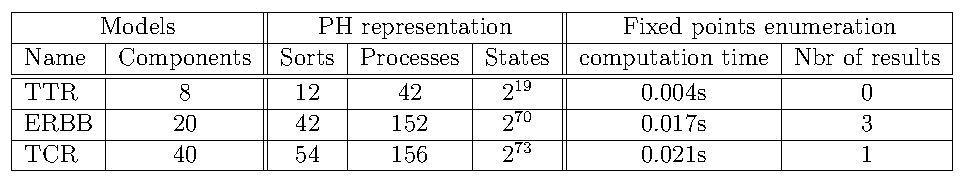
\includegraphics[width=\textwidth]{images/table1.pdf}
\caption{\label{tab:models}%
Description of the models used in our tests and results of our fixed point enumeration.
Each model is referred to by its short name, where
TTR stands for the tadpole tail resorption model% ~\cite{khalis2009smbionet},
ERBB for the receptor-regulated G1/S transition of the same name% ~\cite{Samaga2009}
and TCR for the T-cell receptor signaling network %\cite{Klamt06}.
For each of them, this table gives the number of biological components
in the original representation,
and the number of sorts, the number of processes
and the number of states in the PH model.
Finally, the last column gives the computation time for the enumeration of all fixed points
and the number of results returned.
}
\end{table}

\begin{table}[ht]
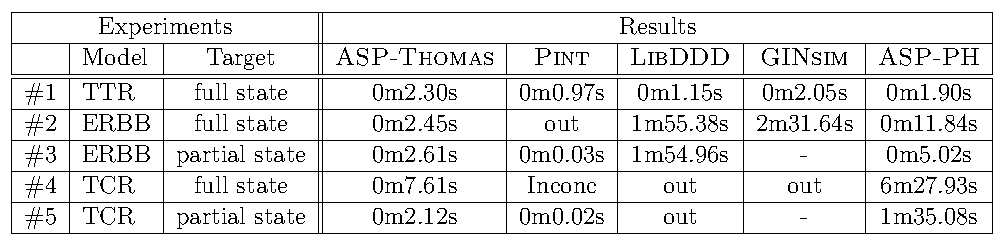
\includegraphics[width=\textwidth]{images/table2}
\caption{\label{tab:reachability}%
Compared performances of several methods to compute reachability analyses:
The method of Rocca \textit{et al.} (denoted by \textsc{ASP-Thomas}), \textsc{Pint}, \textsc{LibDDD}, \textsc{GINsim} and our new method presented in this paper, called \textsc{ASP-PH}.
For each test, this table gives the short name of the considered model,
as given in table~\ref{tab:models},
the type of goal (either a whole state or a sub-state)
and the computation time of the different methods used for the tests,
where “out” marks an execution taking too much time or memory,
\mbox{“~-~”} indicates that is not possible to do the test,
and “Inconc” states that the method terminates without a response.
}
\end{table}

\begin{itemize}

\item \textbf{ASP-Thomas}\footnote{These tests have been performed on another computer: dual core , 2.13 GHZ with 1.8 GB RAM. The authors wish to thank Laurent Trilling for his help.}
offers the possibility to model-check CTL properties of Thomas networks. 
There is no automatic way that allows the modelisation of Thomas networks in ASP. That is why it is necessary to study the entire network than to present it in ASP. But this modelisation takes so much time to be done regarding the complex representation of Thomas networks. Comparing with our method, we use the PH model which its actions are more easy to be presented in ASP, one fact per action.
In addition, the method "ASP-Thomas" requires to provide a maximum number of steps
for which the dynamics will be computed, which mays be difficult to be predicted.
However it is clear that this approach gives a very quick result when compared with others.
Indeed it also show that ASP is a good choice to run the dynamics of a model and check reachability properties. 
Furthermore, this method is able to check any kind of CTL formula
(and not only the “$\mathsf{EF}$” form that we focused on in this paper).
(see the discussion in section~\ref{limitations}).

\item \textbf{\textsc{GINsim}} is a software for the edition, simulation and analysis
of gene interaction networks.
It allows to compute all reachable stable states from a given initial state instantly;
however, it is not possible to compute all stable states independently from the initial state.
Regarding the reachability problem, \textsc{GINsim} only allows to check the reachability of
full states, because its approach consists in computing
all the state-transition graph and then search for a path between the two given states.
Therefore, it was not possible to perform reachability checks on partial states
(experiments \#3 \& \#5).
Small state-transition graphs can also be displayed by this tool.

\item \textbf{\textsc{LibDDD}}
is a library for symbolic model-checking of CTL \& LTL properties.
It can thus especially be used to check reachability properties;
however, as opposed to our method, it does not output an execution path
solving this reachability.
In addition, it relies on the construction of the state-transition graph
which is then stored under the form of a binary decision diagram for a more efficient analysis.
This computation explains why \textsc{LibDDD} takes more time to respond,
and gets out of memory in about 12 minutes for the biggest example
which contains $2^{73}$ states
(experiments \#4 \& \#5).
Finally, \textsc{LibDDD} is not able to compute the stable states of a network.

\item \textbf{\textsc{Pint}}
is a library gathering tools and converters related to the PH.
It should be noted that \textsc{Pint} contains the only reachability analysis
developed so far natively for the Process Hitting,
before the method proposed in this paper.
It consists in an approximation that avoids to compute the state-transition graph;
it is thus ensured to be really efficient, which explains the fastest results,
but at the cost of possibly terminating without being conclusive.
However, it is not designed for goals consisting of many processes,
which are more likely to trigger an inconclusive response
(such as for experiment \#4),
or an exponential research in sub-solutions
(such as for experiment \#2).
This explains the high computation times for some tests in table \ref{tab:reachability}.
Moreover, in the case of a positive answer,
it currently does not return the execution of the path achieving the desired reachability,
but only outputs its conclusion.
\end{itemize}

\subsection{Strengths and limitations of our method}
\label{limitations}

In the previous sections,
we developed new methods in ASP to check dynamical properties,
namely identifying stable states and finding all possible paths to reach a given goal.
Compared to some other methods describes above
(\textsc{GINsim}, \textsc{LibDDD} and the method \textsc{ASP-Thomas}) our method is relatively faster and also permits to study larger networks
(up to $2^{73}$ states in our tests). We study the networks which are modeled in Process Hitting. This new fomalisim for network modelisation is a restriction of synchronous automata so it allows to represent any kind of dynamical model. Moreover it is easy to implement the dynamics of the PH into ASP.
However, our ASP program may still be non-conclusive
in the cases where the given goal is not
reachable and the model contains loops in its dynamics
(which happens in almost every biological model).
In this case, the program will compute all infinite paths in these loops,
and never reach a goal or a fixed point.
It is still possible, however, to limit the number of iterations to an arbitrary
maximum which will be eventually reached in the case of an endless loop.
This is possible with the option \texttt{"-{}-imax=n"} of \textsc{iClingo},
where \texttt{n} is the maximum number of steps.
%%
%\begin{lstlisting}[numbers=none]
%iclingo find\_path.lp <network\_name>.lp -- imax=n
%\end{lstlisting}
%%

Several values can be given to this parameter.
For example, the total number of states is an obvious maximum,
as it will never be exceeded by a minimum path,
but it is too hight to be very interesting.
The total number of sorts is a more interesting value,
under the hypothesis that each one will change its active process at most once,
which is often the case for Boolean networks;
or, with a similar reasoning, the total number of processes can be chosen.
In these cases, however, a termination with no solution cannot be considered as a formal
negative answer, unless one can prove that the chosen value \texttt{n}
is bigger than the longest possible path in the state-transition graph.
Given our implementation, if the step \texttt{n} is reached,
the computation stops and there is no path to be displayed because there is no path which verifies the goals after \texttt{n} changes. Indeed this permits to get a final result, which is \texttt{unsatisfable} property after \texttt{n} steps so with this way we eliminate the unlimitaded execution time.
